\documentclass[11pt, a4paper]{article}

\usepackage{graphicx}
\usepackage[english]{babel}
\usepackage[utf8x]{inputenc}
\usepackage{amsmath}

\usepackage[a4paper,top=3cm,bottom=2cm,left=2cm,right=2cm,marginparwidth=1.75cm]{geometry}
\graphicspath{ {./images} }

\begin{document}

\setcounter{section}{3}
\section{Lecture 3 (20/02/2020)}
\subsection{Primer on polar coordinates}
Describing rotation in cartesian coordinates can be tedious and time consumig. Luckily, polar
coordinates are a thing. Using polar coordinates makes describing motion along a curved path and
rotational motion much easier and faster. Some basic properties and conversion between polar and cartesian
coordinates will be covered below.

\begin{gather}
    (x , y) = (r\cos(\theta), r\sin(\theta))\\
    r = \sqrt{x^2 + y^2}\\
    dA = dxdy = rdrd\theta\\
    \iint_{D}\,dA = \int_{a}^{b} \int_{c}^{d}\,dxdy = \int_{\alpha}^{\beta} \int_{0}^{r} r\,drd\theta
\end{gather}

\subsection{Known path in polar coordinates}
\begin{figure}[h]
    \centerline{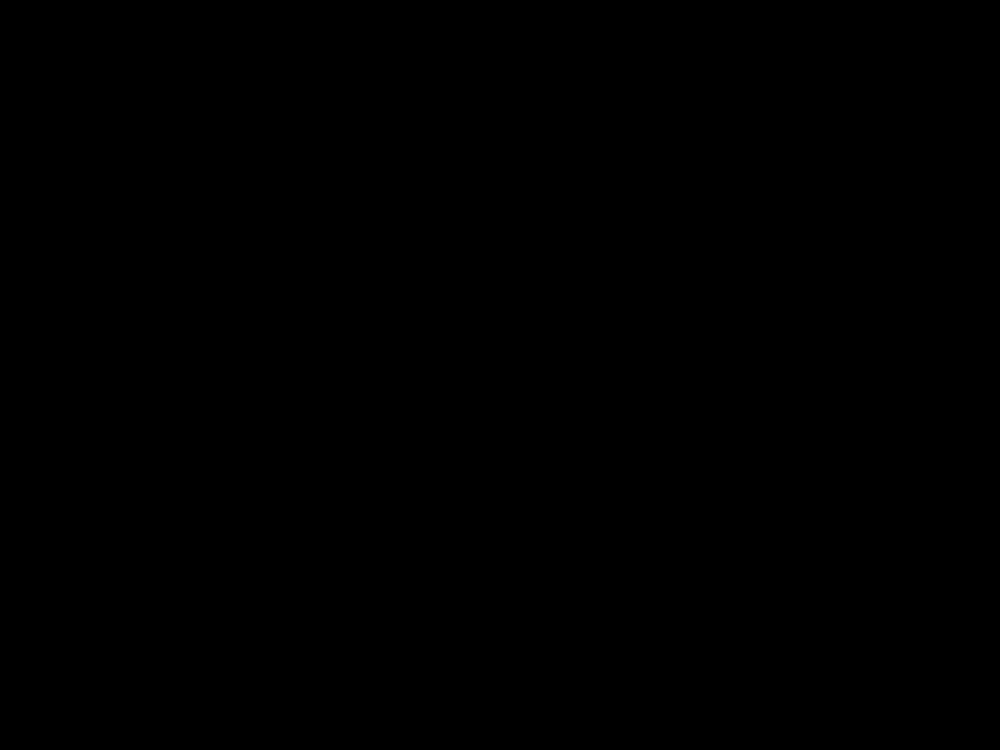
\includegraphics[width=3.5cm]{images/placeholder.png}}
    \caption{Figure placeholder}
\end{figure}

\begin{gather}
\vec{x} = \begin{pmatrix} r\cos(\theta) \\ r\sin(\theta) \end{pmatrix}
    = r \cdot \begin{pmatrix} \cos(\theta) \\ \sin(\theta) \end{pmatrix}\\
    \text{let $\theta = \theta(t)$, $r = r(t)$}\\
    \dot{\vec{x}} = \frac{d\vec{x}}{dt} =  
        \begin{pmatrix} 
            \dot{r}\cos(\theta) - r\sin(\theta) \cdot \dot{\theta}\\
            \dot{r}\sin(\theta) + r\cos(\theta) \cdot \dot{\theta}\\
        \end{pmatrix}
    = \dot{r} \cdot \begin{pmatrix} \cos(\theta) \\ \sin(\theta)\\ \end{pmatrix}
        + r\dot{\theta} \cdot \begin{pmatrix} -\sin(\theta) \\ \cos(\theta)\\ \end{pmatrix}
\end{gather}

It's worth noting that the unit vectors $\boldsymbol{\hat{u}_t}$ and $\boldsymbol{\hat{u}_n}$ for the tangential and perpendicular
components can be recognized in the definition of $\dot{\vec{x}}$. The following definition follows:
\begin{gather}
\boldsymbol{\hat{u}_r} = \begin{pmatrix} \cos(\theta) \\ \sin(\theta)\\ \end{pmatrix} \Rightarrow \text{Perpendicular component}\\
    \boldsymbol{\hat{u}_\theta} = \begin{pmatrix} -\sin(\theta) \\ \cos(\theta)\\ \end{pmatrix} \Rightarrow \text{Tangential component}\\
\end{gather}
Derrivation for $\ddot{\vec{x}}$ can be found in the Hibbeler Dynamics book, I am currently to lazy to look it up and write it out
so you'll just have to believe what I wrote. This gives the following:
\begin{align}
    \begin{cases}
        \vec{x} = r\boldsymbol{\hat{u}_r}\\
        \dot{\vec{x}} = \dot{r}\boldsymbol{\hat{u}_r} + r\dot{\theta}\boldsymbol{\hat{u}_\theta}\\
        \ddot{\vec{x}} = (\ddot{r} - r\dot{\theta}^2)\boldsymbol{\hat{u}_r} + (r\ddot{\theta} + 2\dot{r}\dot{\theta})\boldsymbol{\hat{u}_\theta}\\
    \end{cases}
\end{align}
Side note for equation (11), $\ddot{r} - r\dot{\theta}^2$ and $r\ddot{\theta} + 2\dot{r}\dot{\theta}$ are the components $a_n$ and $a_t$ respectivly

\subsection{Example Problem using polar coordinates with a known path of motion}
A point mass with $m = 0,5\,kg$ moves along the curved path $r = (0,1\theta)\,m/rad$ on the horizontal plane.
let $\theta = \pi\,rad$, $\dot{\theta} = 4\,rad/s$, $\ddot{\theta} = 0\,rad/s^2$
\begin{figure}[h]
    \centerline{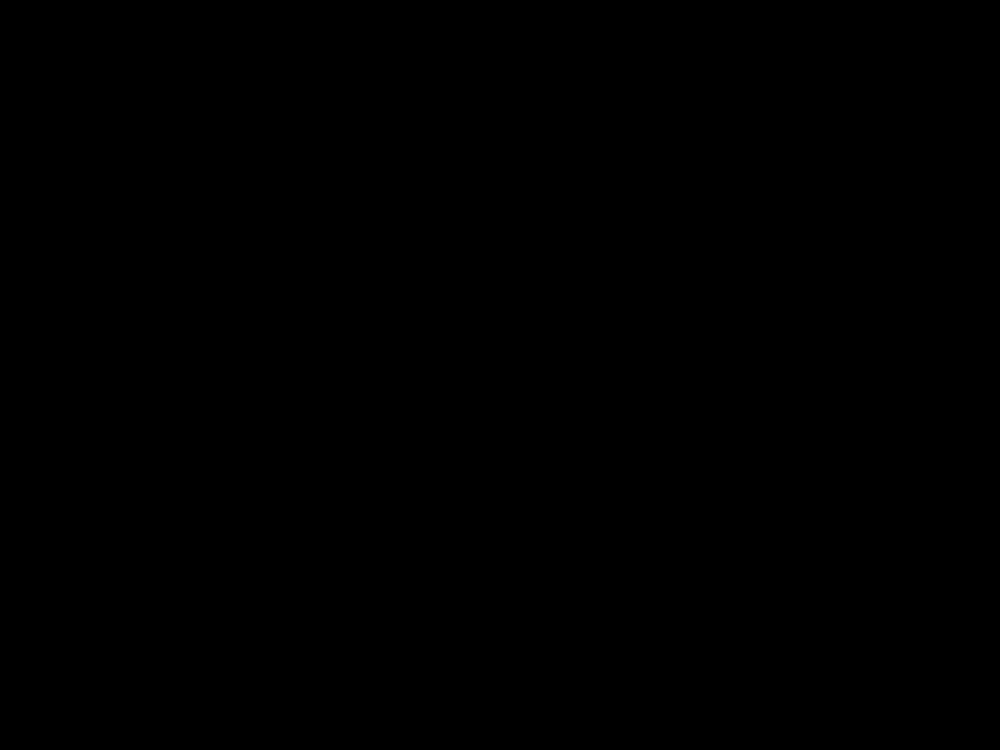
\includegraphics[width=5cm]{images/placeholder.png}}
    \caption{Figure placeholder}
\end{figure}
\setcounter{equation}{0}
\begin{gather}
    \Sigma F_r = -N\cos(\phi) = ma_r\\
    \Sigma F_\theta = F + N\sin(\phi) = ma_\theta\\
    a_r = \ddot{r} - r\dot{\theta}^2 \\
    a_\theta = r\ddot{\theta} + 2\dot{r}\dot{\theta}
\end{gather}
There are now 4 equations, 2 equations of motion and 2 constraint equation. The system has 5 variables
so a new equation needs to be introduced to solve for the angle $\phi$.
\begin{figure}[h]
    \centerline{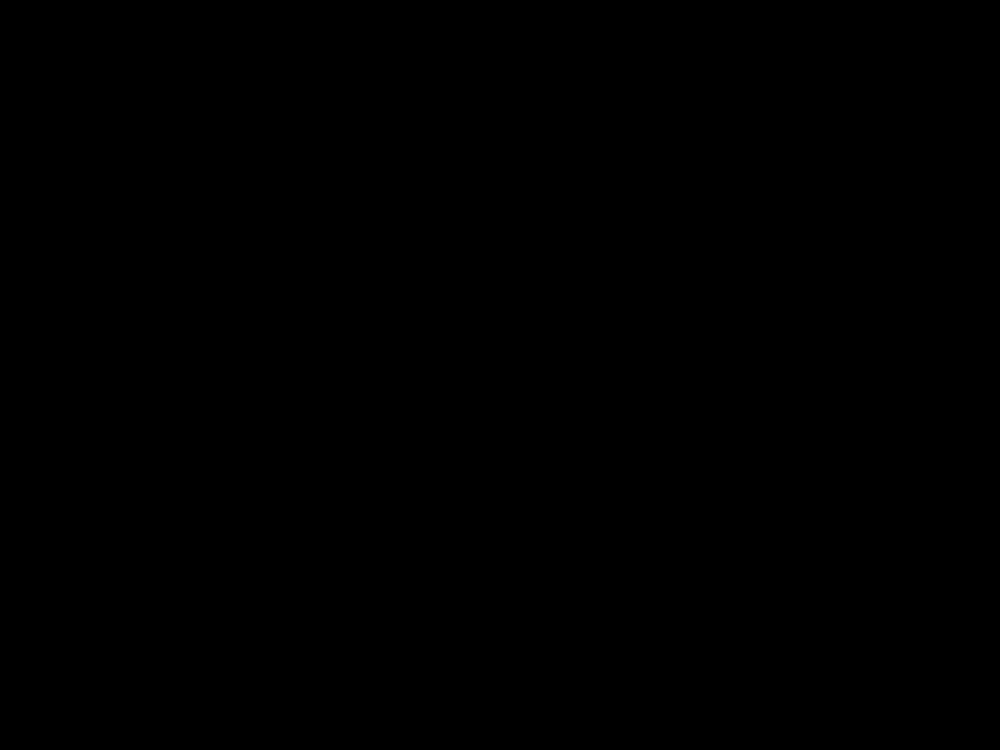
\includegraphics[width=5cm]{images/placeholder.png}}
    \caption{Figure placeholder}
\end{figure}
Looking at the point mass from really close reveals some interesting properties if the angle $\theta$ 
becomes infitesimally small. The line offset from $r$ by $d\theta$ is approximately parrallel to $r$.
This implies that the distance traversed by the particle is $rd\theta$. Using the triangle in 
figure 3 gives the following:
\begin{gather}
    \tan(\phi) = \frac{dr}{rd\theta} = \frac{1}{r} \cdot \frac{dr}{d\theta} \Rightarrow
    \phi = \arctan \left( \frac{1}{r} \cdot \frac{dr}{d\theta} \right)
\end{gather}
This makes equation (5) this fifth and final equation required to solve the problem. It is also possible to
determin the value of angle $\phi$ using a complemantary angle $\psi$. This method is used in the Hibbeler Dynamics book.\\
\\
Using the given information and equation (3) and (4) gives:
\begin{gather}
    a_r = -5,0625\,m/s^2\\
    a_\theta = 3,2\,m/s^2
\end{gather}

For the angle $\phi$ we know the following:
\begin{gather}
    \frac{dr}{d\theta} = \frac{d(0,1\theta)}{d\theta} = 0,1 \\
    \phi = \arctan \left(\frac{1}{\pi} \cdot 0.1 \right) = 0,03182\,rad
\end{gather}

Subsituting the found values from equation (6),(7) and (9) into equation (1) and (2)
gives the following values for $N$ and $F$:
\begin{gather}
    N = \frac{-ma_r}{\cos{\phi}} = 2,53\,N\\
    F = ma_\theta - N\sin(\theta) = 1,52\,N
\end{gather}

Note: Add figures then this is done.
\end{document}
